\textbf{Craftables} Potions and filters can have wondrous effects on experienced alchemists. \\

\begin{tabular}{m{2cm}m{2cm}m{6cm}m{5cm} } \hline
	
\includegraphics[width=2cm]{../Pictures/Gameplay/Items/Consumables/Potions/Antidote_potion_picture.png} & \textbf{Antidote} & Neutralizes poisonous effects from magical creatures. Can be used both in battle and outside. & Ingredients: Bezoar, Standard Ingredient, Unicorn Horn, Mistletoe Berries. \\ \hline
	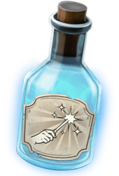
\includegraphics[width=2cm]{../Pictures/Gameplay/Items/Consumables/Potions/Exstimulo_potion_picture.png} & \textbf{Exstimulo Potion} & Increases the power of spells casted in the next 4 turns. & Ingredients: Re'em Blood, Granian Hair, Snowdrop and Bitter Root. \\ \hline
	
\includegraphics[width=2cm]{../Pictures/Gameplay/Items/Consumables/Potions/Felix_felicis_potion_picture.png} & \textbf{Felix Felicis} & Makes who drinks it extremely lucky. Combat rewards are increased, healing potions effect is increased, and all rolls are rolled with advantage. & Ingredients: Ashwinder egg, Squill builb, Murtlap Tentacle, Tincture of thyme, Occamy eggshell, Rue. \\ \hline
	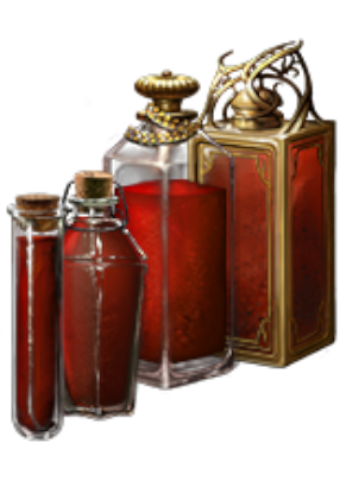
\includegraphics[width=2cm]{../Pictures/Gameplay/Items/Consumables/Potions/Healing_potion_picture.png} & \textbf{Healing Potion} & Recovers health points. This potion's effect varies based on the amount of ingredients used to prepare it. & Ingredients: Rue, Valerian Sprigs and Bitter root \\ \hline
	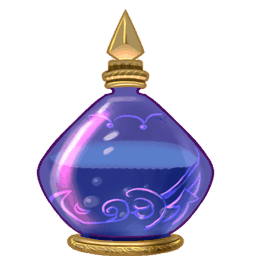
\includegraphics[width=2cm]{../Pictures/Gameplay/Items/Consumables/Potions/Invisibility_potion_picture.png} & \textbf{Invisibility Potion} & Makes the user invisible. In battle the potion lasts 3 turns, out of battle it lasts one minute. The potion affects the user and everything he's carrying; it terminates when the user attacks, casts a spell, or shifts form. & Ingredients: Flobberworm Mucus, Lavender, Valerian Sprigs, Standard ingredient \\ \hline
\end{tabular}

\clearpage

\paragraph {Healing Potion crafting}
The more ingredients are used to craft the healing potion, the stronger is the resulting effect, thanks to an higher concentration of the magical essence.

\begin{tabular}{m{2cm}m{3cm}m{4cm}m{4cm} } \hline
	\textbf{Potion} & \textbf{Quality} & \textbf{HP recovered} & \textbf{Amount of each ingredient} \\ \hline
	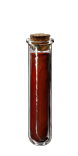
\includegraphics[width=2cm]{../Pictures/Gameplay/Items/Consumables/Potions/Normal_healing_potion_picture.png} & Normal & 2d4+2  & 1  \\ \hline
	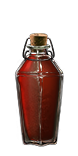
\includegraphics[width=2cm]{../Pictures/Gameplay/Items/Consumables/Potions/Greater_healing_potion_picture.png} & Greater & 4d4+4 & 3 \\ \hline
	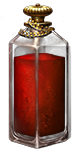
\includegraphics[width=2cm]{../Pictures/Gameplay/Items/Consumables/Potions/Superior_healing_potion_picture.png} & Superior & 8d4+8 & 5 \\ \hline
	
\includegraphics[width=2cm]{../Pictures/Gameplay/Items/Consumables/Potions/Supreme_healing_potion_picture.png} & Supreme & 10d4+20 & 7 \\ \hline
\end{tabular}

\clearpage